\documentclass[12pt]{article}
\usepackage{xeCJK}
\usepackage{tikz}
\usetikzlibrary{calc}
\usetikzlibrary{shapes.geometric}
\usetikzlibrary{positioning}
\usetikzlibrary {arrows.meta}
%\setCJKmainfont{NotoSerifTC-Regular.otf}
%\setCJKmainfont{AdobeMingStd-Light}
%\setCJKmainfont{BiauKaiTC}
\setCJKmainfont{Microsoft JhengHei}

\usepackage{fancyhdr}
\usepackage{lastpage}
\usepackage{amsmath, amssymb}
\usepackage{bm}
\usepackage{graphicx}
\usepackage[all,knot,poly]{xy}
\usepackage{titlesec}
\usepackage{graphicx} % Required for inserting images
\usepackage{algorithm}
\usepackage{algpseudocode}


\pagestyle{fancy}
\renewcommand{\headrulewidth}{0pt}
\fancyhf{}
\lfoot{C802}
\rfoot{page \thepage\ of \pageref{LastPage} pages}
\cfoot{}

\newcommand{\abs}[1]{\lvert#1\rvert}
\newcommand{\e}[1]{\langle {#1}\rangle}
\newcommand{\be}{\begin{equation}}
\newcommand{\ee}{\end{equation}}
\newcommand{\beqn}{\begin{eqnarray}}
\newcommand{\eeqn}{\end{eqnarray}}
\newcommand{\ket}[1]{{| #1 \rangle}}
\newcommand{\bra}[1]{{\langle #1 |}}
\newcommand{\Ket}[1]{{\left| #1 \right\rangle}}
\newcommand{\Bra}[1]{{\left\langle #1 \right|}}
\newcommand{\mean}[1]{{\langle #1 \rangle}}
\newcommand{\ska}[2]{\langle #1 | #2 \rangle}
\newcommand{\skp}[2]{\langle #1 | #2 \rangle}
\newcommand{\trip}[3]{\langle {#1}|{#2}|{#3}\rangle}
\newcommand{\dimer}[1]{\input{#1.latex}}

\titlespacing*{\section}
{0pt}{5.5ex plus .2ex}{4.3ex plus .2ex}
%\titlespacing*{\subsection}
%{0pt}{5.5ex plus .2ex}{4.3ex plus .2ex}


\begin{document}
\noindent
{\bfseries \large 多功能量子退火工具包及其應用}\\
{\bfseries Multifunctional quantum annealing toolkit and its applications}

\section{摘要}
\label{sec: abstract}
模擬退火法、模擬量子退火法、及量子退火法 (又稱絕熱量子計算) 均為物理啟發的全域最佳化方法。
模擬退火法藉熱起伏 (thermal fluctuation) 搜尋解空間,模擬量子退火法建立在路徑蒙地卡羅 (path-integral Monte Carlo),
而量子退火法則由一初始哈密頓算符的基態解出發,藉緩慢改變哈密頓算符達到目標解答。
有鑑於組合最佳化 (combinatorial optimization) 之應用範圍極廣,不同種類的退火運算硬體處理器陸續被建造出,
並能提供實務及商業使用。本計畫將開發綜合上述三類退火演算法以及更多的退火技術之C++軟體套件,
並將參考 D-wave 及Fujitsu Digital Annealer 的使用者介面,以開源軟體方式提供於傳統電腦使用。
除組合最佳化問題的應用,我們所開發的退火工具包也將著重理論物理模型之求解。


\section{研究動機與研究問題}
\label{sec:motivation}

自2023年起我參與使用 Fujitsu Digital Annealer 的專案計畫。
Fujitsu Digital Annealer 是一部以半導體技術建造的退火處理器,
專門處理二次無約束二元最佳化 (quadratic unconstrained binary optimization, QUBO) 問題,
雖然 Fujitsu 標榜其退火處理器使用量子啟發計算 (quantum-inspired computing),
但使用的演算法是不具量子概念的模擬退火法 (simulated annealing) 及平行計算技術。

%%%%%%%%%%%%%%%%%%% FIG %%%%%%%%%%%%%%%%%%%%%%%%%%%%%
\begin{figure}[htp!]
{\par\centering \resizebox*{0.5\textwidth}{!}{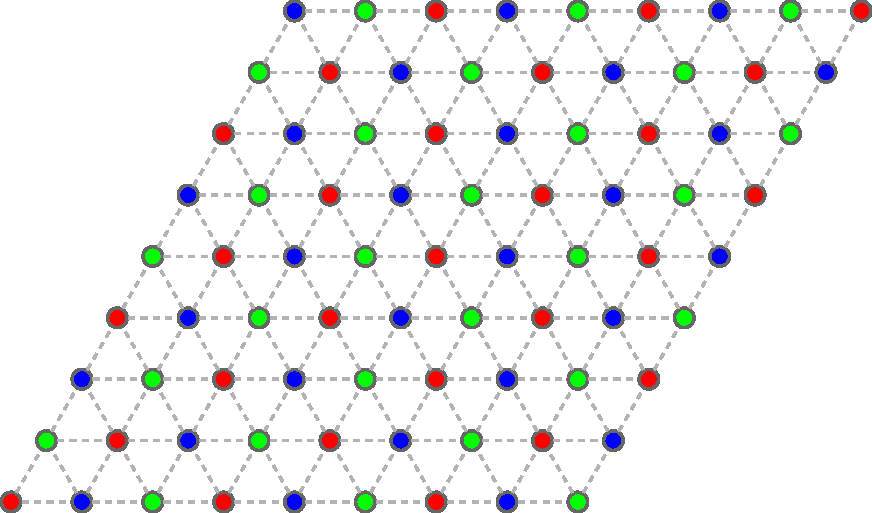
\includegraphics{triangle}} \par}
\caption{
二維三角晶格示意圖。三種不同顏色的晶格代表三個不同的子晶格。
 \label{fig:triangle}
 }
\end{figure}
%%%%%%%%%%%%%%%%%%%%%%

在專題指導教授林瑜琤的指導下,我利用 Fujitsu Digital Annealer 求量子易辛(Ising)自旋三角反鐵磁晶格之基態,
此模型的哈密頓算符(能量算符)定義如下:
\be
   \bm{H}= \sum_{\e{ij}} \bm{Z}_i\bm{Z}_j - h\sum_i \bm{X}_i\,
    \label{eq:qising}
\ee 
其中 $\bm{Z}_i$ 及 $\bm{X}_i$ 分別表示位於晶格點 $i$ 上的 $z$ 及 $x$ 分量的庖立矩陣(Pauli matrix),
$h$ 為指向 $x$ 方向的橫向磁場強度,$\sum$ 下標 $\e{ij}$\ 表示只考慮相鄰的晶格點;
這裡考慮的晶格為如圖Figure~\ref{fig:triangle} 所示的二維三角晶格,由共邊三角形所組成,可以
劃分為三個子晶格 (sublattices)。
在零橫場 $h=0$ 的情形下,此模型為古典(非量子)易辛反鐵磁,其能量值表示為
\be
    H(\{ s_i \}) = \sum_{\e{ij}} s_i s_j\,,
    \label{eq:ising}    
\ee
式中 $s_i$ 為晶格點 $i$ 的二元自旋狀態,可取值 $\{+1,-1\}$ 代表所謂的自旋「朝上」或「朝下」,
如何找出整體自旋的最佳排列使能量值最低為典型的二次無約束二元最佳化 (QUBO) 問題。
以三角晶格的單一三角晶胞來看,任意兩相鄰自旋可滿足反鐵磁性(一朝上,另一朝下 )來達該兩自旋配對的最低能量,
但第三個自旋狀態無論朝上或朝下均會與其中一相鄰自旋的反鐵磁性衝突,
這性質我們稱為幾何挫折性( geometric frustration)。
理論已知~\cite{Wannier,Jiang}  幾何挫折性使零橫場的古典易辛三角反鐵磁甚至在絕對零度下也不具反鐵磁性。
有趣的是,雖然橫場如同溫度傾向破壞有序,在有限橫場下 ($h\neq 0$) 易辛三角反鐵磁反而產生低溫的反鐵磁性,
這是所謂的 order-by-disorder 現象~\cite{Moessner}。
為了得以在 Fujitsu Digital Annealer 上求解帶有橫場的量子自旋模型,
我們藉由Trotter-Suzuki 展開式~\cite{Textbook} 將二維的量子模型轉換成堆疊的三維古典模型~\cite{Moessner},
多出的維度之長度相當於溫度的倒數 $\beta=1/T$。這個等效的三維古典模型也同樣具 QUBO 形式。
圖 Figure~\ref{fig:m} 展示 $h=0$ 及 $h=0.6$ 的序參數分佈情形,這裡序參數定義為以下複數形式~\cite{Moessner}:
\be
    %m\,e^{i\theta}\equiv \left(m_A+m_B\,e^{i(4\pi/3)}+m_C\,e^{i(-4\pi/3)} \right)/\sqrt{3}\,,
     m \equiv \left(m_A+m_B\,e^{i(4\pi/3)}+m_C\,e^{i(-4\pi/3)} \right)/\sqrt{3}\,,
     \label{eq:m}
\ee
其中 $m_\alpha,\,\alpha=A,B,C$為三子晶格(圖 Figure~\ref{fig:triangle})分別的$z$-軸磁化量。
我們確實可觀察到 $h=0$ 模型的序參數集中在 $\abs{m}=0$,代表無有序的反鐵磁性,
而 $h=0.6$ 模型的序參數分佈則集中於 $\abs{m}=0.4$ 附近,呈現反鐵磁性。
值得一提的是,若增加系統的尺度-----包含三角晶格的邊長 $L$ 及針對 $h\neq 0$ 情形的三維等效模型的堆疊高度,
結果將更吻合理論結果,這是所謂的有限系統效應。
對於古典極限下的 $h=0$ 模型,Fujitsu Digital Annealer 確實可以極具效率地提供最佳解答。
可惜受限於 Digital Annealer 所提供的 10 萬個位元數目 (相當於古典自旋數目) 及單次計算容許的最高30分鐘計算時間,
需要更多位元數目的量子模型 ($h\neq 0$) 可執行的系統尺度則有限。

%%%%%%%%%%%%%%%%%%% FIG %%%%%%%%%%%%%%%%%%%%%%%%%%%%%
\begin{figure}[htp!]
{\par\centering \resizebox*{0.75\textwidth}{!}{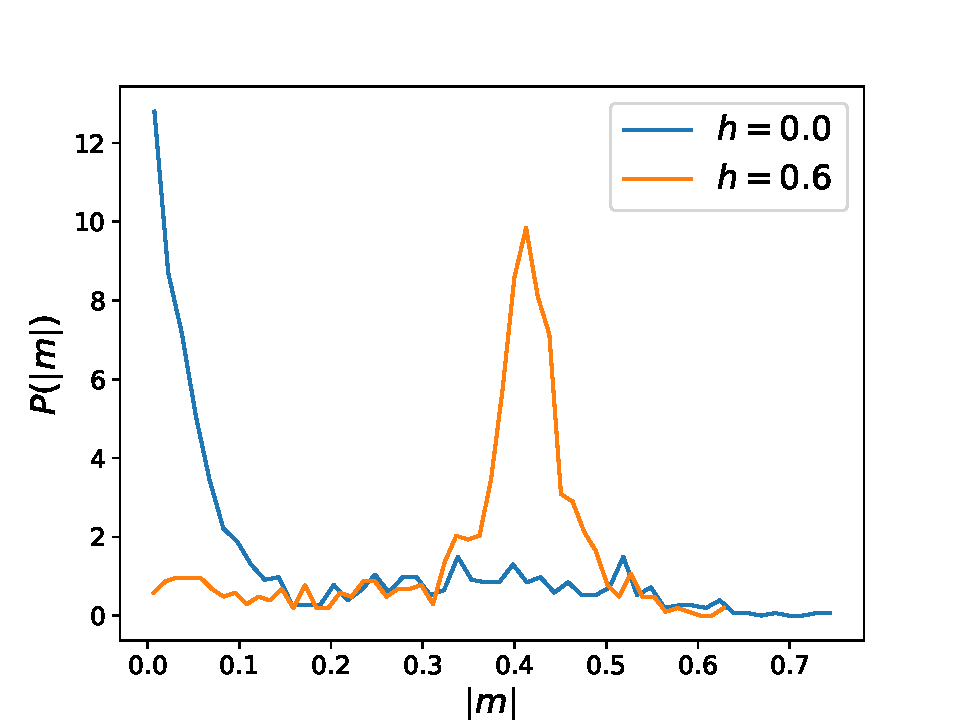
\includegraphics{m.pdf}} \par}
\caption{
 \label{fig:m}
邊長為 $L=21$ 的三角反鐵磁之序參數分佈,此為應用 Fujitsu Digital Annealer 的計算結果,
對兩不同的 $h$ 值各採集 1024 樣本數。針對 $h=0.6$ 的三維等效模型,堆疊的層數共 64 層。
%Distributions of the order parameter $\abs{m}$ for $L=21$ with $h=0$ and $h=0.6$.
 }
\end{figure}
%%%%%%%%%%%%%%%%%%

為克服上述困難,且為了更徹底瞭解量子退火及古典模擬退火的演算法,我開始撰寫這些演算法的程式。
在林瑜琤老師的指導下,我學習到「退火法」有一些不同的類型~\cite{Sandvik_Nat,Huang},
而且均可以用隨機的方式作運算,即所謂的(量子)蒙地卡羅方法;
而量子蒙地卡羅方法也牽涉不同種類的演算法,這些均在我的程式撰寫清單上。
我們也將結合量子退火及古典模擬退火兩種退火路徑~\cite{He},並將之擴充並延伸。

我將開發的退火工具包將以 C++ 語言為進行運算的主要程式,
處理的問題將包含二次無約束二元最佳化問題,及建構在多型態晶格的量子自旋模型。
二次無約束二元最佳化問題可以下列式子表示:
\be
       \min_{\bm{x}}  f(\bm{x}) = \bm{x}^T \bm{Q} \bm{x} + \bm{c}^T \bm{x}  
       \label{eq:qubo}
\ee
式中$\bm{x}^T$ 為一每個元素 $x_i\in \{0,1\}$ 之 $N$ 維列向量,$\bm{Q}$ 為 $N\times N$ 實對稱矩陣,
$c^T$ 為$N$ 維列實向量,目標在於找出最佳的$\bm{x}$ 使得目標函數 $f(\bm{x})$ 達最小值
(也可透過 $-\bm{Q}$ 及 $-\bm{c}$ 轉換成求最大值的問題)。
對於自旋相關的問題,我們習慣將 $\bm{x}$ 的二元值轉換成 $s_i \in  \{-1,+1\}$,轉換式為 $s_i = 2 x_i +1$。
因為我們使用的量子退火演算法起源於處理量子自旋模型,所開發的退火工具包也將適用解決超越上述的二次無約束二元最佳化問題,
能進一步探索量子系統。     

\section{文獻回顧與探討}

%\begin{itemize}
%\item[{\bf 1.}] 模擬退火法 (Simulated Annealing, SA)
%\item[{\bf 2.}] 模擬量子退火法 (Simulated Quantum Annealing, QSA)
%\item[{\bf 3.}] 量子退火法 (Quantum Annealing, QA)
%\item[{\bf 4.}] 隨機級數展開法 (Stochastic Series Expansion)
%\item[{\bf 5.}] 副本交換 (Replica Exchange) / 平行退火 (Parallel Tempering)
%\end{itemize}


\section{研究方法及步驟}
本計畫的執行重點為開發退火工具包,來求解量子易辛模型及任意 QUBO 問題。
以下簡略闡述將納入工具包的演算法:
%\begin{itemize}
%\item[{\bf 1.}] 模擬退火法 (Simulated Annealing, SA)
%\item[{\bf 2.}] 模擬量子退火法 (Simulated Quantum Annealing, QSA)
%\item[{\bf 3.}] 量子退火法 (Quantum Annealing, QA)
%\item[{\bf 4.}] 隨機級數展開法 (Stochastic Series Expansion)
%\item[{\bf 5.}] 副本交換 (Replica Exchange) / 平行退火 (Parallel Tempering)
%\end{itemize}

\subsection*{模擬退火法 (Simulated Annealing, SA)}
此方法模擬物理的退火過程,即將材料加熱然後使之緩慢冷卻的過程,極度緩慢冷卻可減少缺陷產生,即降低系統的能量。
1983年由 Kirkpatrick 等人將這個方法結合 Metropolis 蒙地卡羅的模擬,應用在組合最佳化問題。
以 QUBO 問題為例, 

\subsection*{Algorithm}

\begin{algorithm}
\caption{Simulated Annealing}\label{alg:SA}
\begin{algorithmic}
    \State $s \gets s_0$
\While {$k =0$ through $k_{max}$ (exclusive)}:
    \State $T \gets temperature(~ 1 - \frac{k+1}{k_{max}} ~)$
    \State Pick a random neighbour, $s_{new} \gets neighbour(s)$
\If{$P(~E(s), E(s_{new}~),~T) \geq {random}(0, 1$)} 
    \State $s \gets s_{new}$
\EndIf
\EndWhile
    \State Output: the final state: $s$
\end{algorithmic}
\end{algorithm}

\begin{algorithm}
\caption{Replica Exchange}\label{alg:cap}
\begin{algorithmic}
\Require $myrank \geq 0$, $cmpSrc$, $deltaSFunc$
\State $src_a \gets 0$, $src_b \gets 0$
\State $src_a \gets myrank$, $src_b \gets myrank$ \Comment{Initialize $src_a \& src_b$}
\State $isSwap$ = $false$ \Comment{Initializa $isSwap$ to $false$}
\If{$myrank$ is even}
    \State $src_b \gets myrank + 1$
\Else
    \State $src_a \gets myrank - 1$
\EndIf

\If{$myrank = src_a$} \Comment{$src_b$ will decide whether change the config or not}
    \State Send $cmpSrc$ to $src_b$
    \State Receive $isSwap$
    \If{$isSwap$}
        \State send config to $src_b$ \& receive the config from $src_b$
    \EndIf
\ElsIf{$myrank = src_b$}
    \State Receive $cmpSrc$ from $src_a$ as $cmpSrc_a$
    \State $isSwap = cmpSrc(cmpSrc_a, cmpSrc_b, deltaSFunc)$ 
    \State \Comment{$deltaSFunc$ is the function to determine the swap probability}
    \State Send $isSwap$
    \If{$isSwap$}
        \State send config to $src_b$ \& receive the config from $src_b$
    \EndIf
\EndIf

\If{$isSwap$}
    \State Update the config
\EndIf

\end{algorithmic}
\end{algorithm}

在執行進度上,我已完成模擬退火法、部分完成模擬量子退火法及平行退火的程式,
也已建構使用者輸入 QUBO 問題的格式,包含二元變數 $\{+1, -1\}$ 及 ${0 , 1}$ 的轉換。 


\section{預期結果}

本計畫開發的退火工具包因為針對二次無約束二元最佳化問題設計,可應用的範疇很廣,
除了前面敘述的物理模型,還可列舉圖形切割問題、.....

基於我作專題研究的經驗,
實際執行 Fujitsu Digital Annealer 的經驗,有執行 D-wave 計算的可能性(林老師參與的專案計畫),
及我主修資訊科學系所培養的撰寫電腦程式之能力,
我有信心在林老師繼續指導下能開發出具有科學深度且能造福廣大應用者的多功能量子退火工具包。
期待能獲國科會補助我執行這個資訊科學與物理學的跨域研究計畫。

\section*{需要指導教授指導內容}


\begin{thebibliography}{99}
\bibitem{Textbook}
M.~.L.~Bellac, F.~Mortessagne, G.~G.~Batrouni, {\it Equilibrium and Non-Equilibrium Statistical Thermodynamics},
pages 431-435, Cambridge University Press; 1st edition (2004)
\end{thebibliography}
%#############################
%\bibitem{Dwave}
%D-wave systems, inc.,
%\newblock \url{http://www.dwavesys.com/}.

\end{document}
